%\section{Graph-based Representation Learning for Contextualized Embeddings for Code Changes}

\section{Graph-based, Contextualized Embeddings for Code Changes}
\label{embedding:sec}

\begin{figure*}[t]
	\centering
	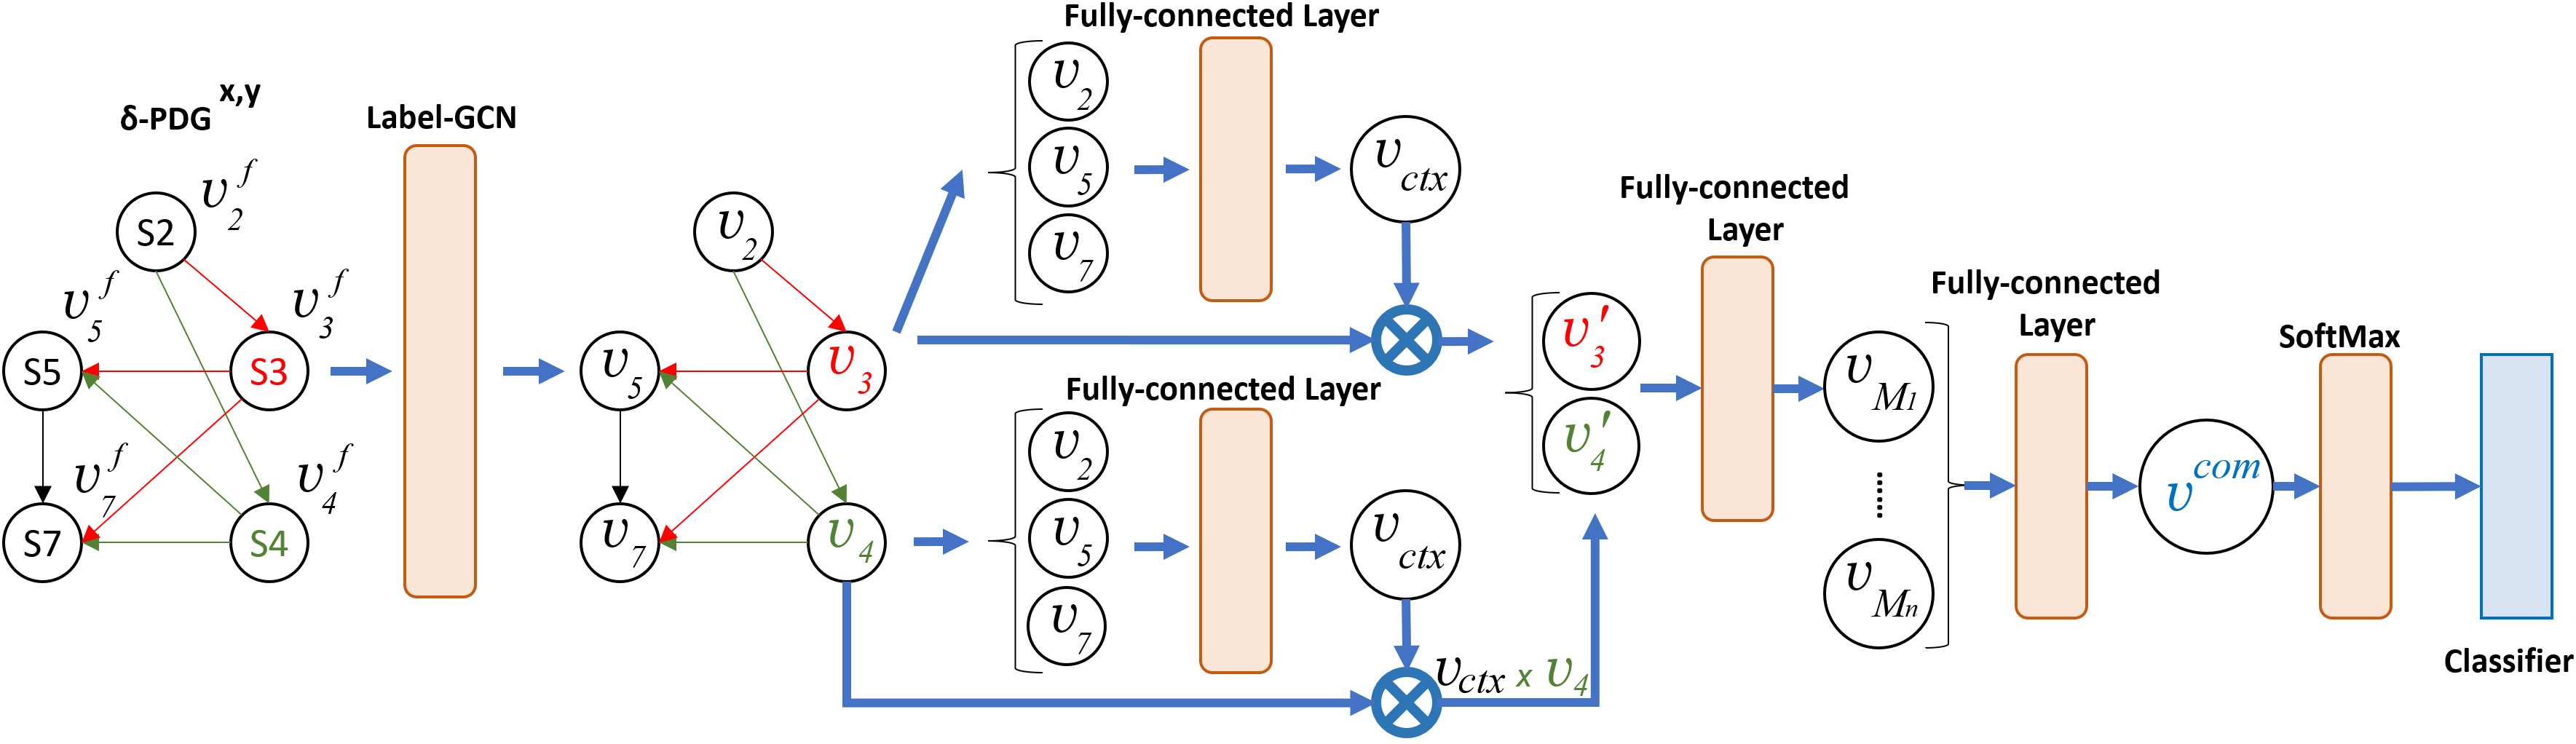
\includegraphics[width=5.8in]{graphs/model-4.png}
	\vspace{-10pt}
	\caption{Context-aware, Graph-based Representation Learning for Contextualized Embeddings for Code Changes}
	\label{fig:step-2}
\end{figure*}

The goal of our representation learning model is to build the {\em
  code change contextualized embeddings} that integrate both {\em
  program dependencies and contexts}.  From those embeddings, {\tool}
builds the embedding for the entire commit, which will be used in the
classification tasks for detection and assessment.

%After the previous step, we obtain the {\mvpdgxy} and the context
%sub-graphs for the changed nodes in {\mvpdgxy}.
%In this step, {\tool} aims to learn the vector/embedding to represent
%the code changes in a commit.
%The embeddings are used to train a model to learn the classifications
%of the commit for a specific vulnerability assessment type.

%with the code change context in the last step, in this step, the goal is to learn the representation vector for code changes in a commit and use the learned representation vector to do the classification for a specific vulnerability assessment type. The key point of the code change representation learning is {\em contextualized} which includes the influence of surrounding source code and the dependency relationships.

\subsection{Feature Vectors $v^{f}_n$ for {\mvpdgxy} Nodes}
\label{feature:sec}

After the previous step, we obtain {\mvpdgxy} and the context
sub-graphs for the changed nodes in {\mvpdgxy}. We leverage
Label-GCN~\cite{label-gcn} to model {\mvpdgxy} as follows. We first
build the node feature vector for each node $n$ in {\mvpdgxy}. To do
so, we use the sequence of the code tokens $t_n$ of the statement $s$
corresponding to $n$. We use a word embedding
model to learn the vector $v_t$ for each token when we consider the
code token sequence for $s$ as a sentence. The {\em node content
  vector} for $n$ is computed as the average vector $v_{avg}$ of
all the vectors $v_t$ of all the tokens in the statement $s$.
%We compute the average vector $v_{avg}$ of all the vectors $v_t$ of
%all the tokens in the statement $s$, and consider $v_{avg}$ as the
%{\em node content vector}.
%
To integrate the labels $x$, $y$, and ($x,y$) into the node feature,
we use a one-hot vector with the length of 3 for those labels. By
concatenating the node content vector with the one-hot vector for the
labels, we have the {\em node feature~vector $v^{f}_n$} for the node
$n$. 

%To obtain the vectors for the nodes in the $\delta$-PDG, we need: (a)
%statement node vector, (b) feature vector, (c) Label-GCN. Each
%statement node in the $\delta$-PDG is essentially a sequence of code
%tokens. We obtain its vector (a) by taking an average of the GloVe
%embeddings for all tokens in the code sequence. Next, we obtain the
%feature vector incorporating the label information in a node, i.e.,
%(b) which is a one-hot vector of the version labels
%(lines_537_549). Concatenating (a) and (b) gives the vectors for the
%nodes in the $\delta$-PDG that is fed into the Label-GCN, which
%through Equations (1)-(3), generate the vector/embedding for each node
%in $\delta$-PDG.


%No need for this para
%To achieve that, we first use the Label-GCN \cite{label-gcn} to model
%{\mvpdgxy}. The first advantage of using Label-GCN is its ability to
%capture the dependencies among the statements represented by the
%nodes. The second advantage comes from the ability to support and
%consider the labels during the computing the vectors of the nodes. We
%use the label mechanism in Label-GCN to represent the labels for the
%versions $x$ and $y$. Specifically, the label $x$ is for a deleted
%node, $y$ for an inserted node, and ($x,y$) for an un-changed node.

\subsection{Contextualized Embedding $v_n$ for Node $n$}
\label{label-gcn-compute}

Next, we replace each node $n$ in {\mvpdgxy} with the node feature
vector~$v^{f}_n$.
%and feed the graph to the Label-GCN to generate the embedding $v_n$
%for each node~$n$.
Similar to the traditional GCN~\cite{gcn}, Label-GCN~\cite{label-gcn}
takes the graph with the node feature vectors as the input and
generates the embeddings for each node in the graph. In addition, for
the current node, in the first layer, Label-GCN considers the change
labels of the neighboring nodes as part of the feature vectors.
%it accepts the node labels in the first layer to better integrate the
%features from the neighboring nodes based on the known labels. To
%consider the label information, it takes the labels of the neighboring
%nodes into account as parts of the features of neighboring
%nodes.
Label-GCN generates the representation vectors (embeddings) for the nodes in each
layer as follows:
\begin{equation}\label{eq1}
	H_{(l)} = 
	\begin{cases}
		\sigma [(\hat{A}X-diag(\hat{A})\sum_{j=1}^{K}e_je^T_j)W^0] &  l = 1\\
		\sigma (\hat{A}H^{(l-1)}W^{(l-1)}) &  l \geq 1\\
	\end{cases}
\end{equation}
\begin{equation}\label{eq2}
	\hat{A} = \tilde{D}^{-\frac{1}{2}}\tilde{A}\tilde{D}^{-\frac{1}{2}}
\end{equation}
\begin{equation}\label{eq3}
	\tilde{A} = A + I
\end{equation}
Where $H$ is the output for hidden layers; $A$ is the
adjacency~matrix and $I$ is the identity matrix; $\tilde{D}$ is the diagonal node degree matrix; $W$
is the weight matrix; $X$ is the input and $X \in R^{num \times (d+K)}$;
$num$ is the number of nodes;~$d$ is the dimension of node features;
$K$ is the number of types of node labels in the input ($K$=3 for $x$,
$y$, and ($x,y$)); and $-diag(\hat{A})\sum_{j=1}^{K}e_je^T_j$ is used
to eliminate the self-loops for the components of the feature vectors
for the labels.

The vectors $H(l)$ at the output layer are used as the vectors $v_i$s
for the nodes in the {\mvpdgxy} graph after Label-GCN in Figure~\ref{fig:step-2}.



%Those feature vectors and the connections among the nodes in
%{\mvpdgxy} will be fed into the Label-GCN model.

%To make the Label-GCN can work on the incoming {\mvpdgxy}, \tool firstly generates the node feature vector for each node $n$ in the {\mvpdgxy}. To do that, \tool regards the content of each node $n$ (the content is the statement) as a sequence of token $t_n$ and then uses the GloVe \cite{} to learn the embedding vector $v_t$ for each token. Then \tool uses the average vector $v_{avg}$ for all token embedding vectors $v_t$ in node $n$ as the node content vector. To combine the label information $x$, $y$, and $x, y$ for each node into the node feature, \tool uses a one-hot vector with a length of $3$ to represent the label. By concatenating the node content vector with the one-hot vector for the label, each node $n$ in {\mvpdgxy} will have the node feature vector $v_{n}^{fea}$. Next, we feed the {\mvpdgxy} with the node feature vector for each node $n$ together to the Label-GCN to generate the representation vector $v_n$ for all nodes in the graph.

\subsection{Integrating Context and Building the Vector for a Commit}
\label{class:sec}

For each changed node $n_c$ in {\mvpdgxy}, we build the sub-graph
containing all the un-changed nodes in the $k$-hop neighbors of $n_c$
and use that sub-graph as the context for $n_c$. We merge the vectors $v_i$s
in the context into a matrix. We then use a fully connected layer on
the matrix to build the {\em context vector $v_{ctx}$} for
the context.

To integrate the context into the embeddings, we compute the final
vector $v{'}_{n_{c}}$ for the changed node $n_c$ by performing the
cross-product between $v_{ctx}$ and the vector $v_{n_c}$ for $n_c$
computed by the Label-GCN model as described in
Section~\ref{label-gcn-compute}:$v{'}_{n_c} = v_{ctx} \times
v_{n_c}$.
To compute the vector for the entire commit, we collect all
the vectors $v{'}_{n_c}$s of the changed nodes $n_c$ in {\mvpdgxy}
into a matrix. We apply a fully connected layer to learn
the vector $v_{Mi}$ for a changed method $Mi$. The vectors for all changed
methods are passed through another fully connected layer to get the
vector $v^{com}$ for the commit. This vector is fed
into each SoftMax classifier for each task.

%To generate the representation vector for code changes in a commit, \tool first collects all representation vectors for the unchanged nodes in its $k$-hop neighbors for each changed node $n_c$ in graph {\mvpdgxy}. And then \tool uses a fully connected layer to learn the vector $v_{ctx}$ representing the context of the changed node $n_c$ by using the merged matrix that is built with all collected representation vectors as the input. Next, \tool calculates the final representation vector $v'_{n_c}$ by using the cross product to combine the representation vector $v_{n_c}$ for Label-GCN and $v_{ctx}$. After this, to consider on the whole commit level, \tool puts all representation vector $v'_{n_c}$ for the changed nodes $n_c$ in {\mvpdgxy} as a matrix, and then apply the other fully connected layer to learn the final vector $v^{com}$ for the entire commit. By having the commit-level representation vector $v^{com}$, \tool uses a SoftMax layer as the classifier to classify the commit for a specific type of vulnerability assessment. As for the details for all types of vulnerability assessment, we will introduce them in the next step.

\subsection{Illustrating Example}

Figure~\ref{fig:step-2} illustrates the vector building for the code
changes in Figure~\ref{fig:multi-version-pdg}. From
{\mvpdgxy}, we compute the node feature vectors $v^{f}_n$
(Section~\ref{feature:sec}) for all statement nodes $S_2$,...,$S_7$ in
that graph. Label-GCN takes that graph with node feature vectors to
generate the embeddings $v_2$,..., $v_7$ for the nodes
(Section~\ref{label-gcn-compute}).

%Figure \ref{fig:step-2} shows the procedure of contextualized embeddings for code changes step by using the case in Figure \ref{fig:multi-version-pdg} as an example. In the Figure, $S_2$, ..., $S_7$ are the statements in $Line-2$, ..., $Line-7$. The \tool uses Label-GCN takes the {\mvpdgxy} as input for Label-GCN model to generate the representation vectors for each node ($V_2$, ..., $V_7$).

Let us consider the changed nodes, $n_3$ and $n_4$. The context for
$n_3$ with one-hop distance includes $n_2$, $n_5$, and
$n_7$. Similarly, the context for $n_4$ includes the same nodes. After
merging those vectors into a matrix, which is passed through a
fully-connected layer, we obtain the context vectors $v_{ctx}$ for
$n_3$. Similarly, we obtain $v_{ctx}$ for $n_4$. Then, the final
contextualized vector for the changed node $n_3$ taking the context
into account is computed as the cross-product: $v'_3$ = $v_{ctx}$
$\times$ $v_3$. Similarly, $v'_4$ = $v_{ctx}$ $\times$ $v_4$.
%
We then put the vectors $v'_3$ and $v'_4$ together in a matrix and use
a fully-connected layer (FCL) to produce the method vector
$v_{M1}$.~All changed method vectors are passed through another FCL to
get $v^{com}$ for the commit. Finally, we pass $v^{com}$ to a SoftMax
layer to perform vulnerability detection or the classification for an
assessment type (e.g., {\em None}, {\em Partial}).

%Then for the changed nodes ($S_3$ and $S_4$), \tool collects the 1-hop neighbors for each of them including $V_2$, $V_5$, and $V_7$. By merging these vectors into a matrix and passing through the fully-connected layer, \tool gets the $V_{ctx}$ for $V_3$ and $V_4$ separately

%(The context for changed statements could be different. The 1-hop context for $V_3$ and $V_4$ are the same just a special case.). And then, by using the cross product to combine $V_{ctx}$ with $V_3$ and $V_{ctx}$ and $V_4$, we have $V'_3$ and $V'_4$.

%By putting them together as a matrix and passing it into the other fully-connected layer, \tool gets the representation vector $V^{com}$ for the entire commit. In the end, \tool passes the $V^{com}$ to a SoftMax layer to do the classification for the vulnerability assessment.
